\chapter{Screenshots of the Application}
\label{app:screenshots}

This section contains screenshots of the working artefact.

\begin{figure}[H]
    \centering
    
\includegraphics[width=\textwidth]{figures/Figure_13_Final_Home_Page.png}
    \caption{Home Page}
    \label{fig:final_home_page}
\end{figure}

\begin{figure}[H]
    \centering
    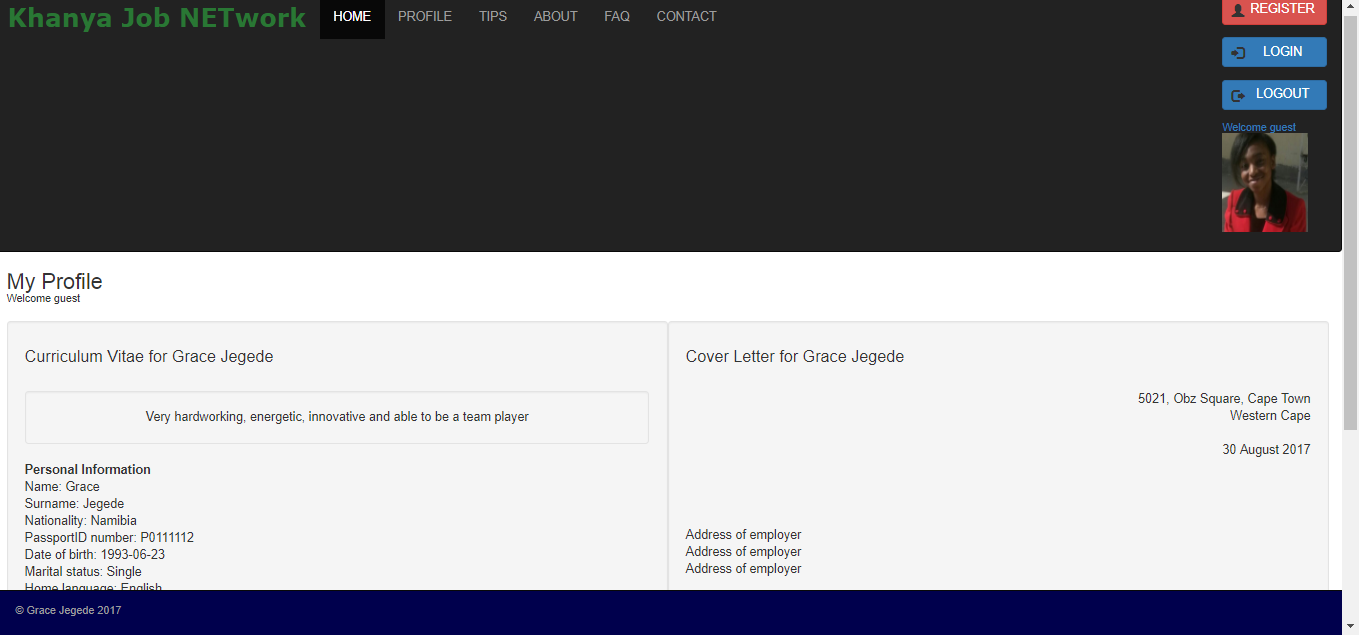
\includegraphics[width=\textwidth]{figures/Figure_14_Profile_Page.png}
    \caption{Profile Page}
    \label{fig:profile_page}
\end{figure}

\begin{figure}[H]
    \centering
    \includegraphics[width=\textwidth]{figures/Figure_15_Tips_Overview_Tiles_Page.png}
    \caption{Tips Overview Tiles Page}
    \label{fig:tips_overview_tiles}
\end{figure}

\begin{figure}[H]
    \centering
    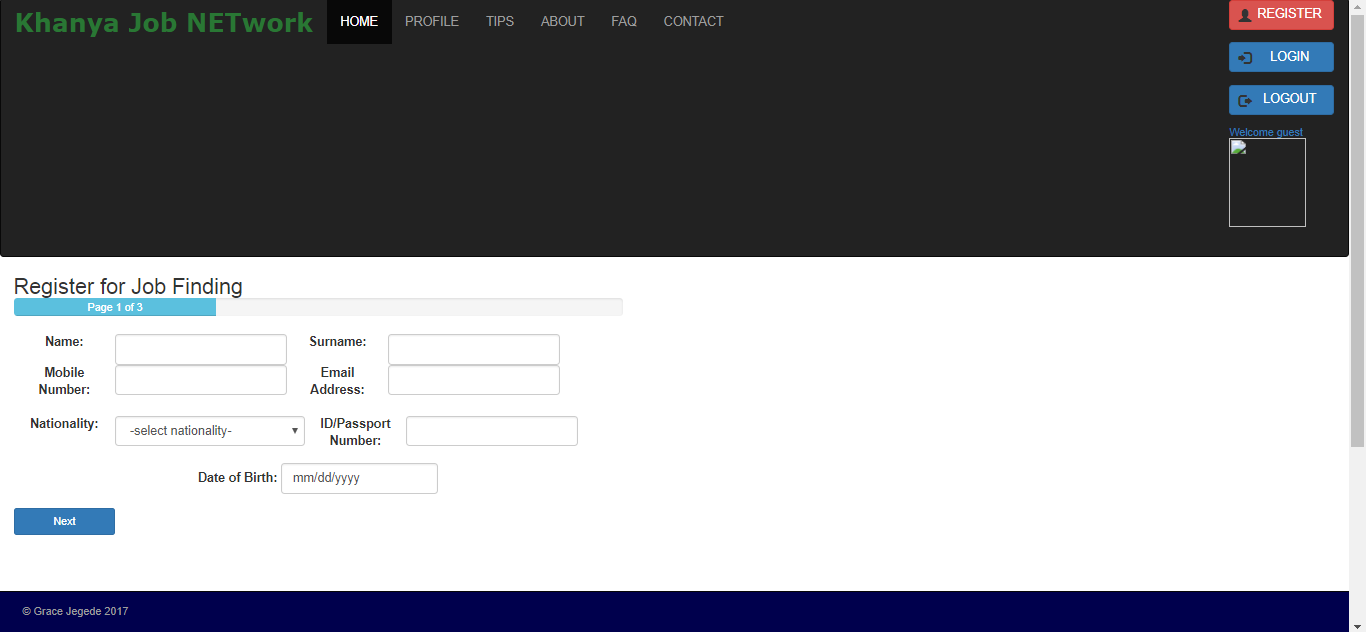
\includegraphics[width=\textwidth]{dissertation/figures/Figure_16_Registration_Page1_of_3.png}
    \caption{Registration Page 1 of 3}
    \label{fig:registration_page1}
\end{figure}

The registration page has three forms with progress indicated with a progress bar. The progress bar shows the user whether they are on page 1 of 3, 2 of 3 or 3 of 3.

\begin{figure}[H]
    \centering
    
\includegraphics[width=\textwidth]{figures/Figure_17_Progress_Bar.png}
    \caption{Progress Bar}
    \label{fig:progress_bar}
\end{figure}

\begin{figure}[H]
    \centering
    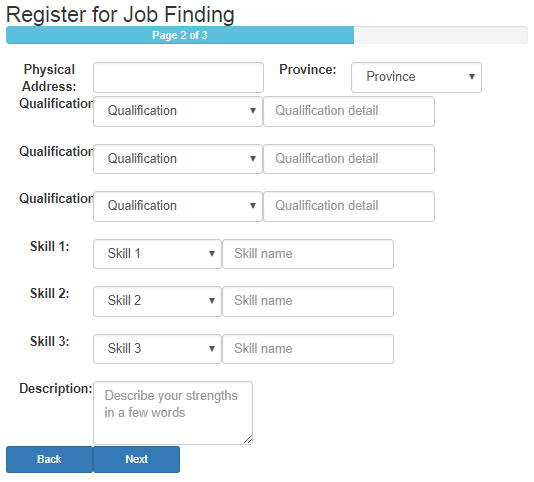
\includegraphics[width=\textwidth]{figures/Figure_18_Registration_part_2_of_3.png}
    \caption{Registration page 2 of 3}
    \label{fig:registration_page2}
\end{figure}

\begin{figure}[H]
    \centering
    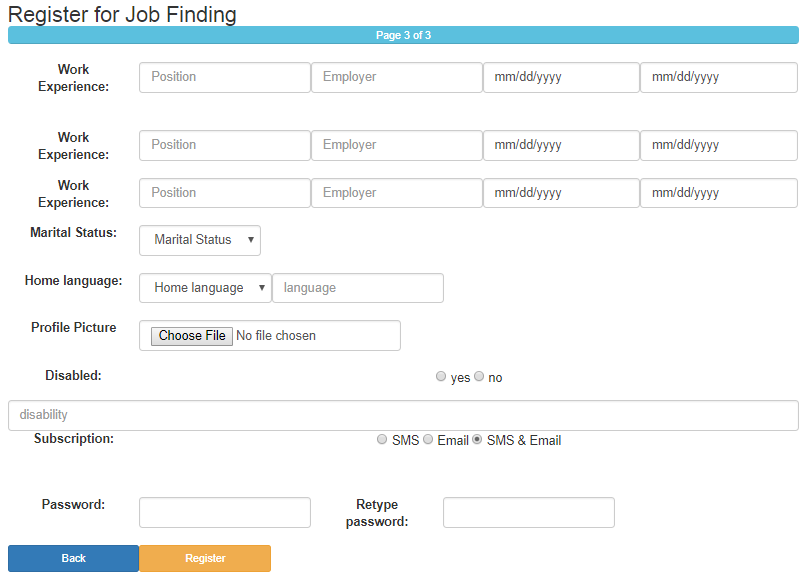
\includegraphics[width=\textwidth]{figures/Figure_19_Registration_part_3_of_3.png}
    \caption{Registration page 3 of 3}
    \label{fig:registration_page3}
\end{figure}

\begin{figure}[H]
    \centering
    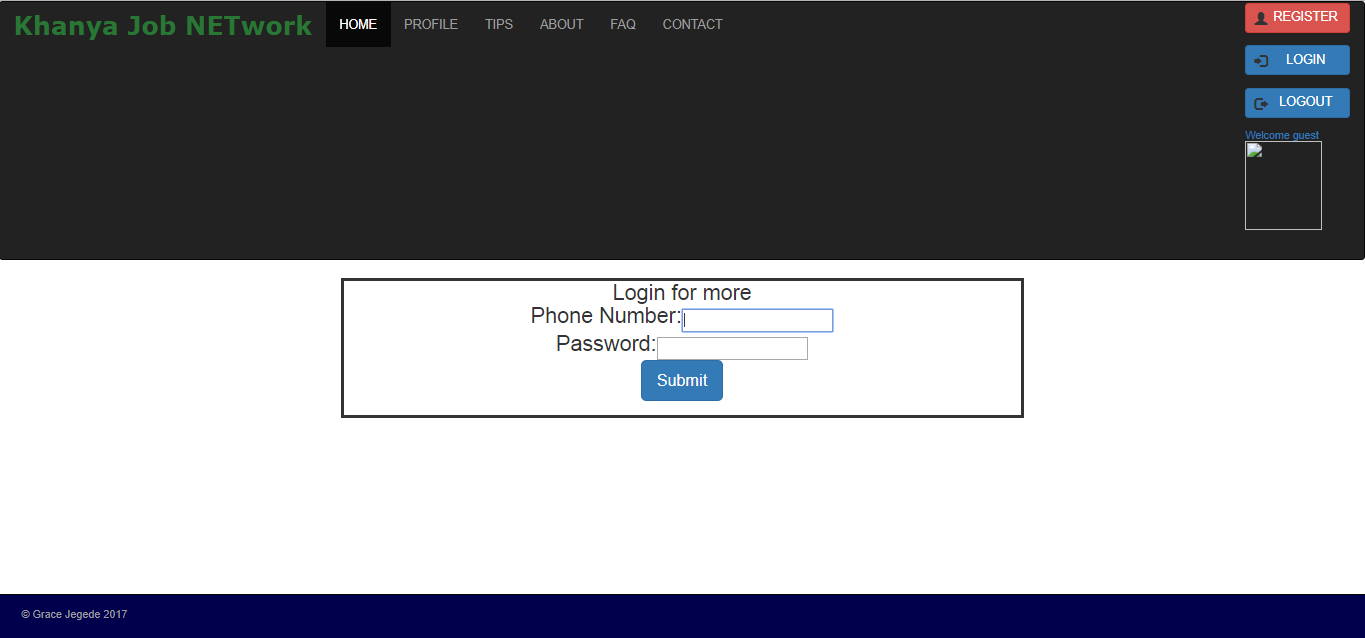
\includegraphics[width=\textwidth]{figures/Figure_20_Login_page.png}
    \caption{Login Page}
    \label{fig:login_page}
\end{figure}

\begin{figure}[H]
    \centering
    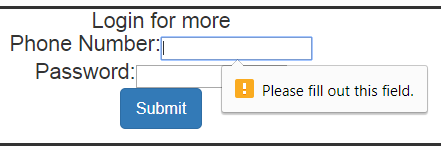
\includegraphics[width=\textwidth]{figures/Figure_21_Section_of_the_Login_page.png}
    \caption{Section of the Login Page}
    \label{fig:login_section}
\end{figure}

An alert message lets a user know a field is not completed if the user tries to submit the page without the required information.

\begin{figure}[H]
    \centering
    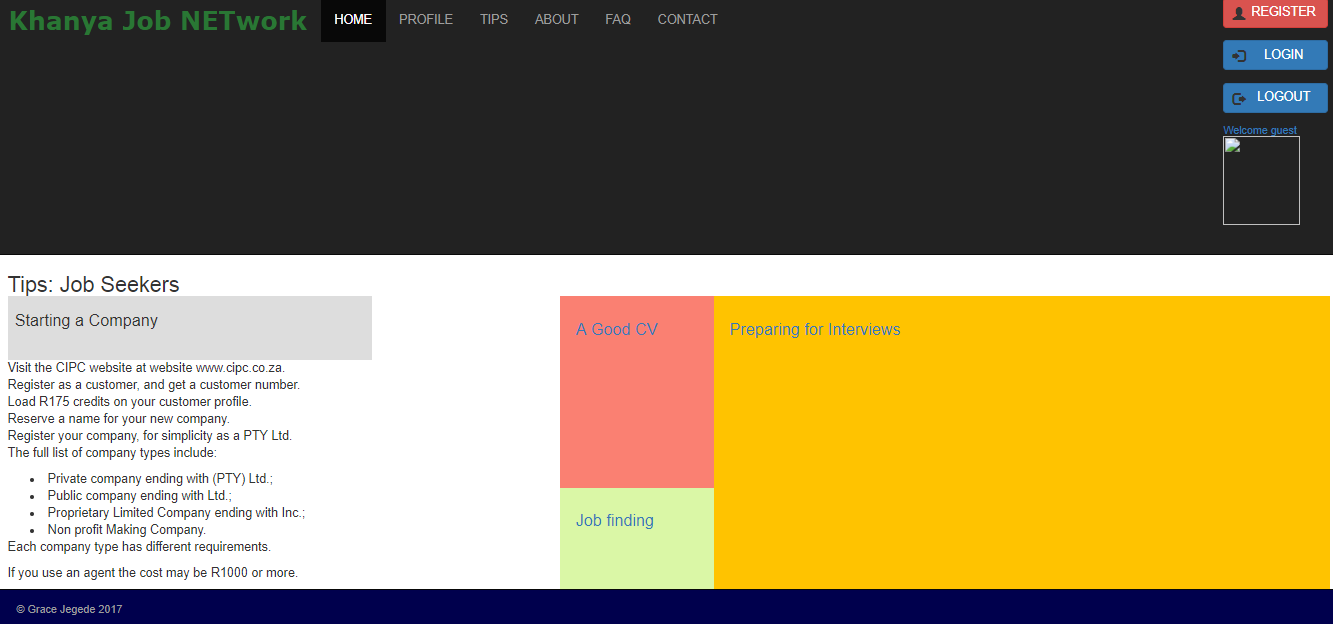
\includegraphics[width=\textwidth]{dissertation/figures/Figure_22_Tips_4_Page_on_Starting_a_company.png}
    \caption{Tip 4: Page on Starting a Company}
    \label{fig:tips_registering_company}
\end{figure}